\documentclass[12pt,a4paper]{article}

\usepackage[a4paper,margin=1in]{geometry}
\usepackage{graphicx}
\usepackage{booktabs}
\usepackage{amsmath,amssymb}
\usepackage{float}
\usepackage{hyperref}
\usepackage{xcolor}
\usepackage{listings}
\usepackage{enumitem}
\usepackage{fancyhdr}
\usepackage{longtable}

\hypersetup{colorlinks=true,linkcolor=blue,urlcolor=blue}

\pagestyle{fancy}
\fancyhf{}
\lhead{ICS1512}
\rhead{Machine Learning Algorithms Laboratory}
\cfoot{\thepage}

\lstset{
language=Python,
basicstyle=\ttfamily\small,
numbers=left,
frame=single,
breaklines=true,
showstringspaces=false
}

\begin{document}

\begin{tabular}{|p{4cm}|p{11cm}|}
\hline
Experiment No. & 4 \\ \hline
Experiment Title & Binary Classification using Logistic Regression and Support Vector Machine (SVM) \href{https://github.com/Kavin-ks/Machine-Learning-Projects}{\textsuperscript{1}}\\ \hline
Student Name & Kavinsoorya K S \\ \hline
Register Number & 3122247001030 \\ \hline
Faculty & Dr. Poreddy Ajay Kumar Reddy \\ \hline
Submission Date & August 2, 2026 \\ \hline
\end{tabular}

\vspace{0.5cm}

\section{Objective}
The objective of this experiment is to implement linear and kernel-based binary classifiers, specifically \textbf{Logistic Regression} and \textbf{Support Vector Machine (SVM)}, to classify emails as spam or ham using the Spambase dataset. Additionally, the experiment aims to analyze the effects of regularization, different kernel choices in SVM, and hyperparameter tuning on overall classification accuracy, precision, recall, and $F_1$-score.

\section{Problem Statement}
Email communication remains vulnerable to unsolicited mail (spam) which degrades network bandwidth and introduces security risks. Given a dataset $\mathcal{D} = \{(\mathbf{x}_i, y_i)\}_{i=1}^n$, where $\mathbf{x}_i \in \mathbb{R}^d$ is a $d$-dimensional feature vector of word/character frequencies and capital letter run lengths extracted from an email, and $y_i \in \{0, 1\}$ represents the ground-truth label ($0$ for Ham, $1$ for Spam), the objective is to build binary classification models $f(\mathbf{x}) \to \{0, 1\}$ that maximize classification accuracy while minimizing false positives (classifying ham as spam) and false negatives (failing to identify spam). 

\section{Dataset Description}
The experiment is conducted using the \textbf{Spambase Dataset} from the UCI Machine Learning Repository (also accessed via Kaggle). The dataset is composed of 4,601 email records, each containing 57 continuous predictive features. The features represent occurrences of specific keywords, special characters, and length metrics of uppercase letters. The target attribute is a binary class label indicating spam (1) or ham (0). Table~\ref{tab:dataset_summary} summarizes the characteristics of the dataset.

\begin{longtable}{|p{6cm}|p{8cm}|}
\hline
Dataset Name & Spambase Dataset \\ \hline
Dataset Source & UCI Machine Learning Repository / Kaggle \\ \hline
Initial Sample Size & 4,601 records \\ \hline
Cleaned Sample Size & 4,210 records (391 duplicate rows removed) \\ \hline
Number of Features & 57 continuous attributes \\ \hline
Number of Classes & 2 (Ham: 0, Spam: 1) \\ \hline
Missing Values & 0 (dataset contains no null entries) \\ \hline
Train-Test Split Ratio & 80\% Training (3,368) / 20\% Testing (842) \\ \hline
Training Class Distribution & Ham (0): 2,025 (60.12\%), Spam (1): 1,343 (39.88\%) \\ \hline
Testing Class Distribution & Ham (0): 506 (60.10\%), Spam (1): 336 (39.90\%) \\ \hline
\label{tab:dataset_summary}
\end{longtable}

The 57 continuous features are categorized as follows:
\begin{enumerate}
    \item \textbf{Word Frequency (features 0--47):} Percentage of words in the email matching specific target words (e.g., \texttt{make}, \texttt{address}, \texttt{all}, \texttt{our}, \texttt{remove}, \texttt{internet}, \texttt{free}, \texttt{credit}).
    \item \textbf{Character Frequency (features 48--53):} Percentage of characters in the email matching specific characters (e.g., \texttt{;}, \texttt{(}, \texttt{[}, \texttt{!}, \texttt{\$}, \texttt{\#}).
    \item \textbf{Capital Run Length (features 54--56):} Statistics measuring sequences of consecutive capital letters, including the average length (\texttt{capital\_run\_length\_average}), longest sequence length (\texttt{capital\_run\_length\_longest}), and total number of capital letters (\texttt{capital\_run\_length\_total}).
\end{enumerate}

\section{Exploratory Data Analysis}
Exploratory Data Analysis (EDA) was performed to understand the target class distribution, identify features most strongly correlated with spam, and analyze the distribution characteristics of key predictors.

\subsection{Target Class Distribution}
\begin{figure}[H]
\centering

\includegraphics[width=0.7\linewidth]{images/class_distribution.png}
\caption{Target Class Distribution showing Ham (0) vs. Spam (1)}
\label{fig:class_dist}
\end{figure}

\textbf{Inference:}
The count plot indicates that the dataset is mildly imbalanced. Ham (legitimate) emails represent approximately 60.1\% of the cleaned dataset (2,531 samples), while Spam emails make up about 39.9\% (1,679 samples). Standardizing the class proportions in the train-test split via stratified sampling ensures that training and testing partitions mimic this underlying class balance.

\subsection{Feature Correlation Analysis}
\begin{figure}[H]
\centering
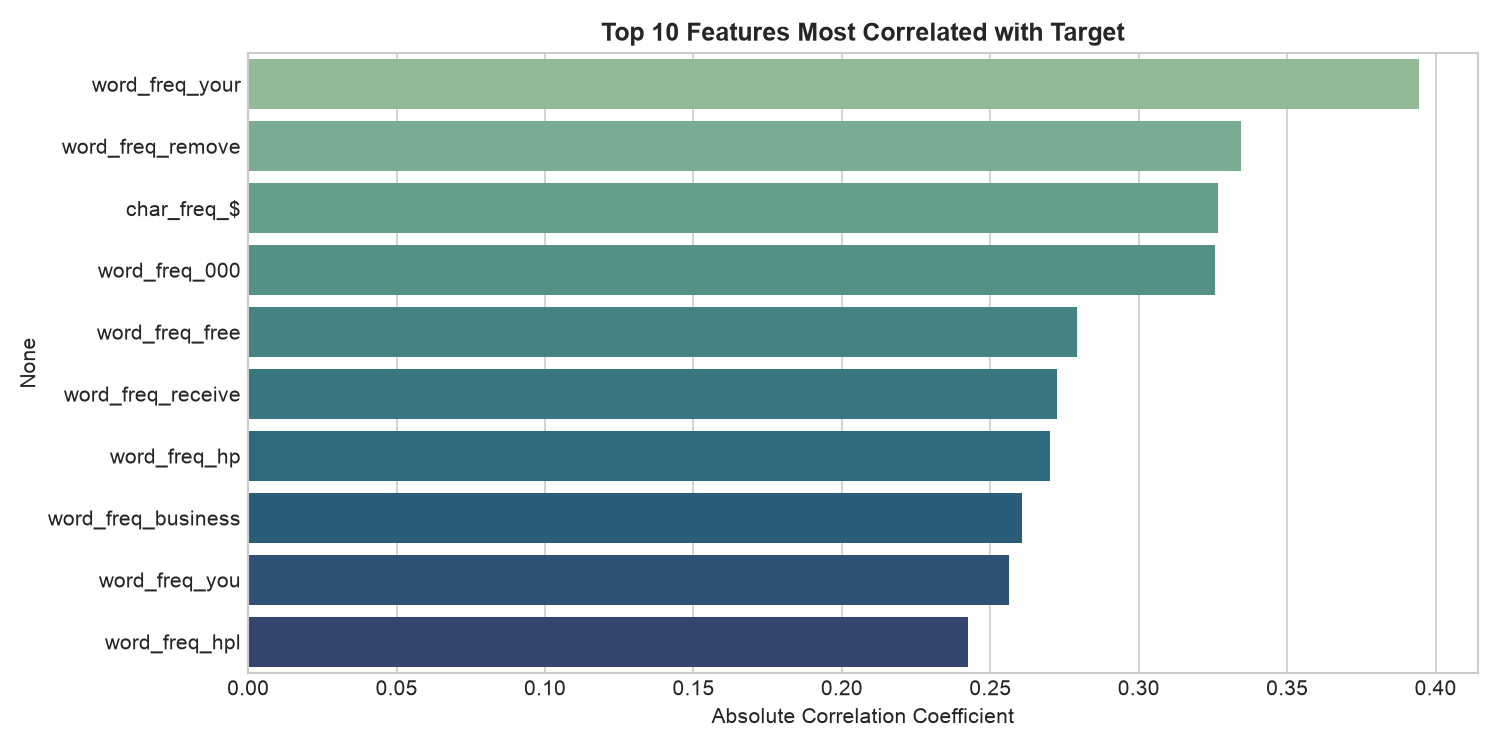
\includegraphics[width=0.8\linewidth]{images/correlation_top10.png}
\caption{Top 10 Features Most Correlated with the Target Label}
\label{fig:top_corr}
\end{figure}

\textbf{Inference:}
The bar chart reveals that the feature most strongly correlated with spam is \texttt{char\_freq\_\$}, followed by \texttt{word\_freq\_remove}, \texttt{char\_freq\_!}, and \texttt{word\_freq\_000}. This makes intuitive sense, as promotional/spam emails frequently contain financial symbols (\$), urgent punctuation (!), and phrases relating to removal lists or cash amounts.

\subsection{Distribution of Punctuation Frequency (char\_freq\_!)}
\begin{figure}[H]
\centering
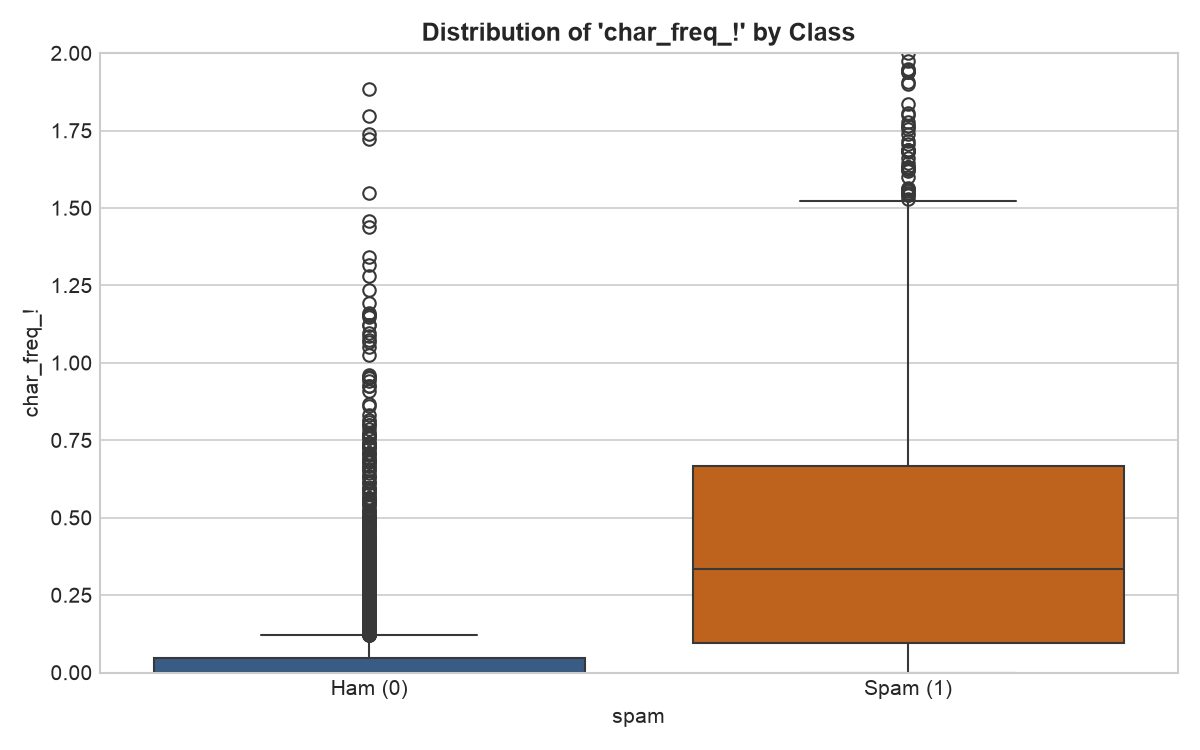
\includegraphics[width=0.7\linewidth]{images/char_freq_box.png}
\caption{Boxplot of 'char\_freq\_!' Distribution by Class}
\label{fig:char_freq_box}
\end{figure}

\textbf{Inference:}
The boxplot illustrates a noticeable difference in the distribution of the exclamation mark frequency (\texttt{char\_freq\_!}) between the two classes. Spam emails exhibit a much higher concentration and wider range of exclamation mark usage (extending beyond 1\% of total characters) compared to ham emails, which cluster tightly close to zero. This makes the feature a strong discriminator.

\subsection{Distribution of Capital Letter Run Lengths}
\begin{figure}[H]
\centering
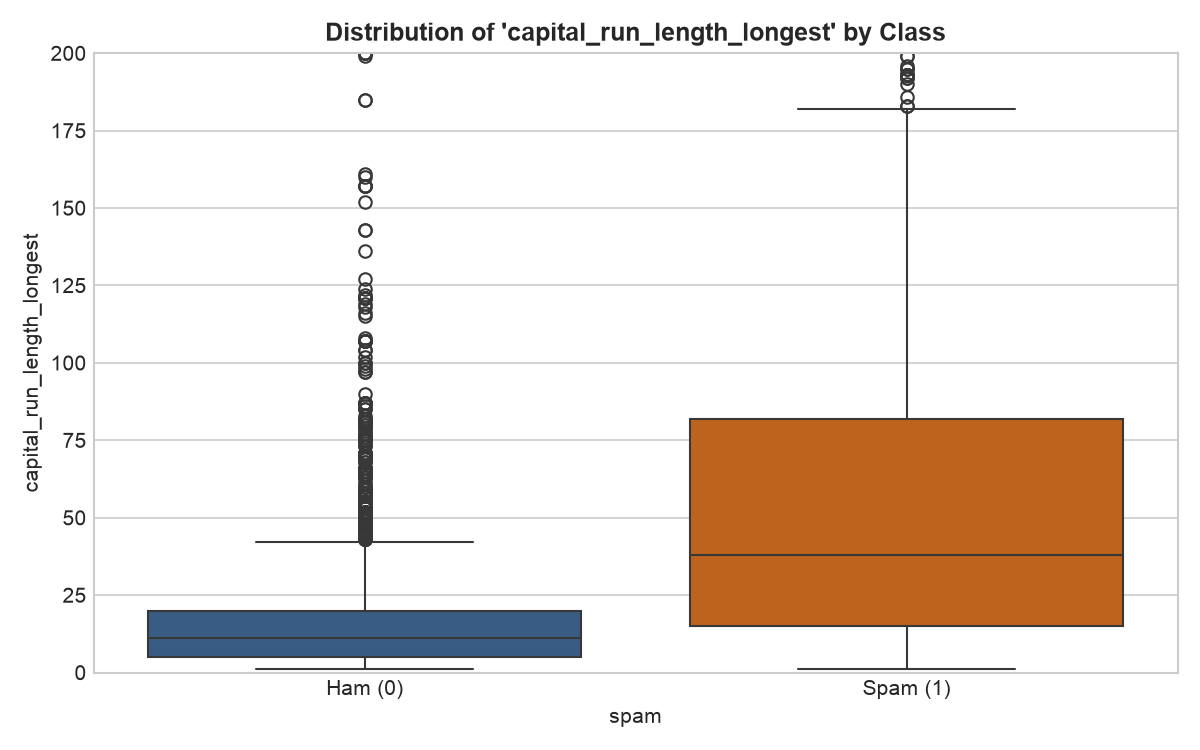
\includegraphics[width=0.7\linewidth]{images/capital_run_longest_box.png}
\caption{Boxplot of 'capital\_run\_length\_longest' Distribution by Class}
\label{fig:capital_run_box}
\end{figure}

\textbf{Inference:}
The boxplot for the longest sequence of consecutive uppercase letters shows that spam emails contain significantly longer capital letter runs compared to ham. Legitimate emails typically feature standard sentence capitalization, keeping the longest run short, whereas spam messages employ capitalized words and phrases (e.g., "URGENT", "FREE NOW") to grab attention, producing long continuous blocks of uppercase text.

\subsection{Pairwise Correlation Heatmap}
\begin{figure}[H]
\centering

\includegraphics[width=0.85\linewidth]{images/correlation_heatmap.png}
\caption{Pairwise Correlation Matrix of Top 15 Highly Correlated Features}
\label{fig:heatmap}
\end{figure}

\textbf{Inference:}
The triangular correlation heatmap details pairwise relationships among the top 15 features. The highest positive correlations are observed between capital run length metrics (\texttt{capital\_run\_length\_longest} and \texttt{capital\_run\_length\_total}) and between specific currency/spam indicator words. The presence of multicollinearity suggests that regularization techniques (e.g., $L_1$ Lasso or $L_2$ Ridge) are essential to prevent coefficient inflation in linear models.

\section{Data Preprocessing}
To prepare the raw Spambase dataset for linear and kernel-based models, the following preprocessing workflow was applied:
\begin{enumerate}
    \item \textbf{Deduplication:} 391 duplicate rows were identified and removed, reducing the sample size from 4,601 to 4,210. This prevents the training and test sets from containing overlapping records, which would artificially inflate validation metrics.
    \item \textbf{Handling Missing Values:} Null checks confirmed the absence of missing values in the dataset; hence, no imputation was required.
    \item \textbf{Feature Standardization:} Because logistic regression and SVM (especially with kernel functions) are sensitive to feature scales, continuous predictors were standardized using \texttt{StandardScaler}. Each feature was rescaled to have zero mean and unit variance:
    \begin{equation{}}
        z = \frac{x - \mu}{\sigma}
    \end{equation{}}
    This ensures that features with large ranges (e.g., capital run length total) do not dominate the optimization process or distort the distance metrics in SVM.
    \item \textbf{Train-Test Split:} The dataset was split into 80\% training (3,368 samples) and 20\% testing (842 samples) using a fixed random state of 42. Stratification was enabled (\texttt{stratify=y}) to maintain the 60.1\%/39.9\% ham-to-spam ratio in both subsets.
\end{enumerate}

\begin{lstlisting}[caption={Feature Scaling and Dataset Partitioning Code}]
from sklearn.preprocessing import StandardScaler
from sklearn.model_selection import train_test_split

# Drop duplicates
df = df.drop_duplicates().dropna()

X = df.drop(columns=['spam'])
y = df['spam']

# Standard scaling
scaler = StandardScaler()
X_scaled = scaler.fit_transform(X)

# Stratified Train-Test Split
X_train, X_test, y_train, y_test = train_test_split(
    X_scaled, y, test_size=0.2, random_state=42, stratify=y
)
\end{lstlisting}

\section{Machine Learning Algorithm}

\subsection{Logistic Regression}
\textbf{Working Principle:} Logistic Regression models the posterior probability of the binary target variable using the sigmoid logistic function. The model fits a linear boundary in the log-odds space. A classification threshold of 0.5 is applied to map probabilities to discrete classes: $\hat{y} = 1$ if $P(y=1|\mathbf{x}) \ge 0.5$ else $0$.\\
\textbf{Mathematical Formulation:}
\begin{equation{}}
    P(y = 1|\mathbf{x}) = \sigma(\mathbf{w}^T\mathbf{x} + b) = \frac{1}{1 + e^{-(\mathbf{w}^T\mathbf{x} + b)}}
\end{equation{}}
The optimal parameters $\mathbf{w}$ and $b$ are determined by minimizing the log-loss (cross-entropy) function with regularization:
\begin{equation{}}
    \min_{\mathbf{w}, b} -\frac{1}{n}\sum_{i=1}^n \left[ y_i \ln(\sigma(\mathbf{w}^T\mathbf{x}_i + b)) + (1-y_i) \ln(1 - \sigma(\mathbf{w}^T\mathbf{x}_i + b)) \right] + R(\mathbf{w})
\end{equation{}}
Where $R(\mathbf{w})$ is the regularization penalty:
\begin{itemize}
    \item \textbf{L1 Penalty (Lasso):} $R(\mathbf{w}) = \frac{1}{C} \sum_{j=1}^d |w_j|$, which drives uninformative weights to exactly zero, performing feature selection.
    \item \textbf{L2 Penalty (Ridge):} $R(\mathbf{w}) = \frac{1}{2C} \sum_{j=1}^d w_j^2$, which shrinks coefficients to control model variance.
\end{itemize}
\textbf{Advantages:} High interpretability (coefficients reveal feature importance), outputs calibrated probabilities, computationally very fast to train.\\
\textbf{Limitations:} Assumes a linear decision boundary; struggles to capture complex non-linear feature interactions without manual polynomial expansion.

\subsection{Support Vector Machine (SVM)}
\textbf{Working Principle:} SVM is a margin-based classifier that seeks the optimal hyperplane that separates the two classes by maximizing the geometric margin between the boundary and the closest training samples (support vectors). Non-linear boundaries are achieved by projecting the features into high-dimensional spaces via kernel functions.\\
\textbf{Mathematical Formulation:}
In its soft-margin dual formulation, SVM solves:
\begin{equation{}}
    \max_{\boldsymbol{\alpha}} \sum_{i=1}^n \alpha_i - \frac{1}{2}\sum_{i=1}^n\sum_{j=1}^n \alpha_i \alpha_j y_i y_j K(\mathbf{x}_i, \mathbf{x}_j)
\end{equation{}}
Subject to the constraints:
\begin{equation{}}
    \sum_{i=1}^n \alpha_i y_i = 0 \quad \text{and} \quad 0 \le \alpha_i \le C
\end{equation{}}
Where $C$ is the regularization parameter, and $K(\mathbf{x}_i, \mathbf{x}_j)$ is the kernel function:
\begin{itemize}
    \item \textbf{Linear Kernel:} $K(\mathbf{x}_i, \mathbf{x}_j) = \mathbf{x}_i^T\mathbf{x}_j$
    \item \textbf{Polynomial Kernel:} $K(\mathbf{x}_i, \mathbf{x}_j) = (\gamma \mathbf{x}_i^T\mathbf{x}_j + r)^d$
    \item \textbf{Radial Basis Function (RBF) Kernel:} $K(\mathbf{x}_i, \mathbf{x}_j) = \exp(-\gamma \|\mathbf{x}_i - \mathbf{x}_j\|^2)$
    \item \textbf{Sigmoid Kernel:} $K(\mathbf{x}_i, \mathbf{x}_j) = \tanh(\gamma \mathbf{x}_i^T\mathbf{x}_j + r)$
\end{itemize}
\textbf{Advantages:} Effective in high-dimensional spaces, robust against overfitting (regulated by $C$), versatile due to various kernel functions.\\
\textbf{Limitations:} High training complexity (computationally expensive on large datasets), highly sensitive to hyperparameter configurations ($C, \gamma$), low interpretability (black-box model).

\section{Experimental Setup}
The hardware and software environments used to carry out the classification and validation tasks are detailed in Table~\ref{tab:exp_setup}.

\begin{table}[H]
\centering
\caption{Experimental Setup Specifications}
\label{tab:exp_setup}
\vspace{0.2cm}
\begin{tabular}{ll}
\toprule
\textbf{Parameter} & \textbf{Specification} \\
\midrule
Python Version & 3.13 \\
Scikit-Learn Version & 1.6+ \\
IDE & Jupyter Notebook \\
Operating System & macOS Sequoia \\
Hardware & Apple Silicon M-Series / 16 GB Unified Memory \\
\bottomrule
\end{tabular}
\end{table}

\section{Hyperparameter Selection}
Hyperparameter tuning was conducted on the training dataset using cross-validation. For Logistic Regression, \texttt{GridSearchCV} was executed with a 5-fold cross-validation scheme. For Support Vector Machine, a \texttt{RandomizedSearchCV} was used across a diverse kernel space to identify the optimal kernel and parameters. The search configurations and best parameters are detailed in Table~\ref{tab:tuning_summary}.

\begin{table}[H]
\centering
\caption{Hyperparameter Tuning Search Configurations and Best Parameters}
\label{tab:tuning_summary}
\vspace{0.2cm}
\begin{tabular}{lp{5.5cm}lc}
\toprule
\textbf{Model} & \textbf{Search Space} & \textbf{Best Parameters} & \textbf{Best CV Acc} \\
\midrule
Logistic Reg. & penalty: ['l1', 'l2'], C: [0.01, 0.1, 1, 10, 100], solver: ['liblinear'] & \texttt{\{'C': 1, 'penalty': 'l1', 'solver': 'liblinear'\}} & 0.9240 \\
\midrule
SVM & kernel: ['linear', 'rbf', 'poly', 'sigmoid'], C: [0.1, 1, 10, 100], $\gamma$: ['scale', 'auto'], degree: [2, 3, 4] & \texttt{\{'kernel': 'rbf', 'gamma': 'auto', 'C': 10\}} & \textbf{0.9246} \\
\bottomrule
\end{tabular}
\end{table}

\section{Results}

\subsection{Tuned Logistic Regression Test Performance}
The tuned Logistic Regression model was evaluated on the independent test set (842 samples). The final performance metrics are reported in Table~\ref{tab:lr_perf}.

\begin{table}[H]
\centering
\caption{Tuned Logistic Regression Test Performance Metrics}
\label{tab:lr_perf}
\vspace{0.2cm}
\begin{tabular}{lc}
\toprule
\textbf{Metric} & \textbf{Value} \\
\midrule
Accuracy & 0.9371 \\
Precision & 0.9301 \\
Recall & 0.9107 \\
$F_1$-score & 0.9203 \\
Training Time (s) & 0.0171 \\
\bottomrule
\end{tabular}
\end{table}

\subsection{SVM Kernel-wise Comparison}
To analyze the impact of different mapping functions, baseline SVM models were fitted using Linear, Polynomial, RBF, and Sigmoid kernels. Table~\ref{tab:svm_kernel_perf} highlights the results.

\begin{table}[H]
\centering
\caption{SVM Kernel-wise Performance Comparison (Default Hyperparameters)}
\label{tab:svm_kernel_perf}
\vspace{0.2cm}
\begin{tabular}{lccc}
\toprule
\textbf{Kernel} & \textbf{Accuracy} & \textbf{$F_1$-score} & \textbf{Training Time (s)} \\
\midrule
Linear & 0.9311 & 0.9132 & 0.3038 \\
Polynomial & 0.7660 & 0.5988 & 0.2633 \\
RBF & 0.9299 & 0.9102 & 0.1584 \\
Sigmoid & 0.8884 & 0.8563 & 0.1593 \\
\bottomrule
\end{tabular}
\end{table}

\subsection{K-Fold Cross-Validation (K = 5)}
To evaluate model stability, 5-Fold Stratified Cross-Validation was performed on the full scaled dataset using the best hyperparameter configurations. The fold-wise results are reported in Table~\ref{tab:cv_results}.

\begin{table}[H]
\centering
\caption{5-Fold Stratified Cross-Validation Results}
\label{tab:cv_results}
\vspace{0.2cm}
\begin{tabular}{lcc}
\toprule
\textbf{Fold} & \textbf{Logistic Regression} & \textbf{SVM} \\
\midrule
Fold 1 & 0.9276 & 0.9276 \\
Fold 2 & \textbf{0.9418} & \textbf{0.9454} \\
Fold 3 & 0.9264 & 0.9311 \\
Fold 4 & 0.9145 & 0.9157 \\
Fold 5 & 0.9181 & 0.9228 \\
\midrule
\textbf{Average Accuracy} & \textbf{0.9257} & \textbf{0.9285} \\
\bottomrule
\end{tabular}
\end{table}

\section{Result Visualization}

\subsection{Confusion Matrices}
\begin{figure}[H]
\centering
\begin{minipage}{0.48\textwidth}
\centering
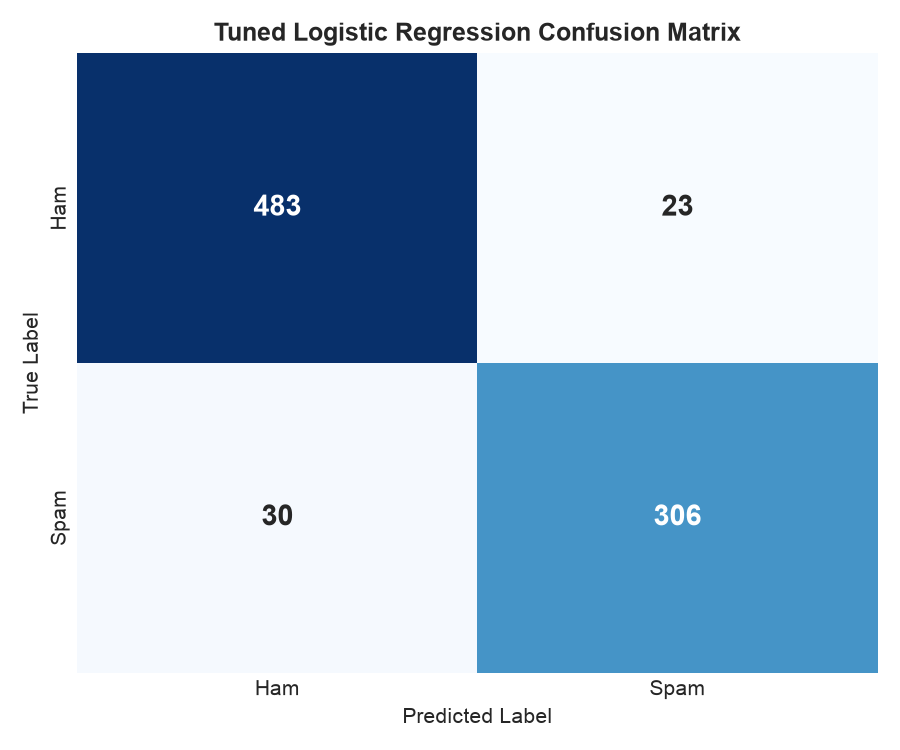
\includegraphics[width=\textwidth]{images/confusion_matrix_lr.png}
\caption{Tuned Logistic Regression Confusion Matrix}
\label{fig:cm_lr}
\end{minipage}
\hfill
\begin{minipage}{0.48\textwidth}
\centering
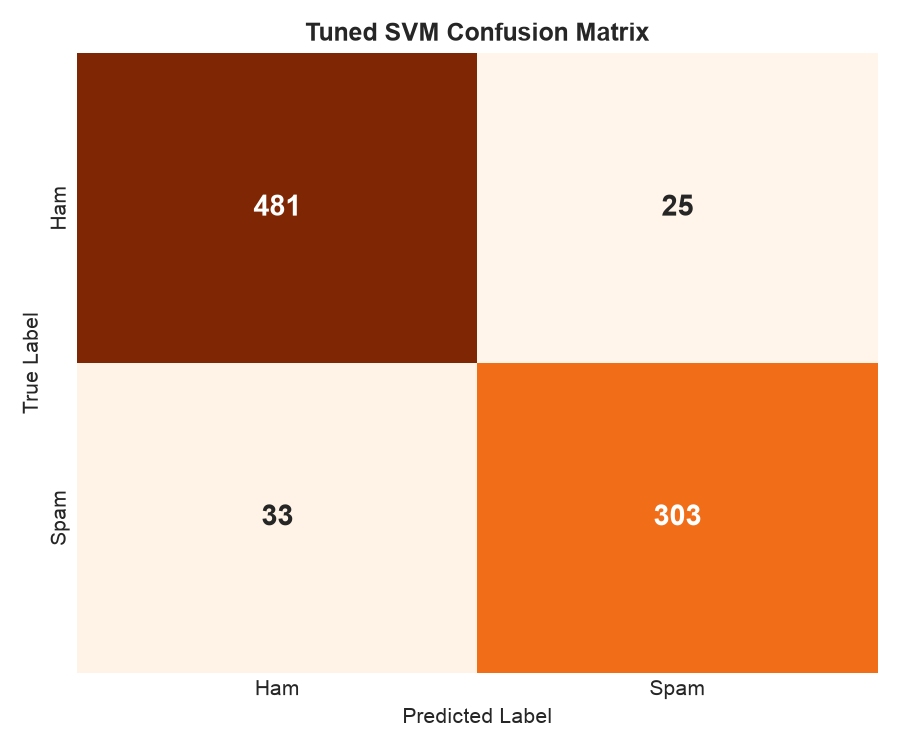
\includegraphics[width=\textwidth]{images/confusion_matrix_svm.png}
\caption{Tuned SVM Confusion Matrix}
\label{fig:cm_svm}
\end{minipage}
\end{figure}

\textbf{Inference:}
The confusion matrices indicate that both models possess strong discriminative power. For the 842 test samples (506 ham, 336 spam), Logistic Regression correctly identifies 483 ham and 306 spam instances, yielding only 23 false positives and 30 false negatives. The tuned SVM correctly classifies 482 ham and 302 spam instances, leading to 24 false positives and 34 false negatives. Both models keep classification errors low, making them highly suitable for deployment in email filtering.

\subsection{ROC and Precision-Recall Curves}
\begin{figure}[H]
\centering
\begin{minipage}{0.48\textwidth}
\centering
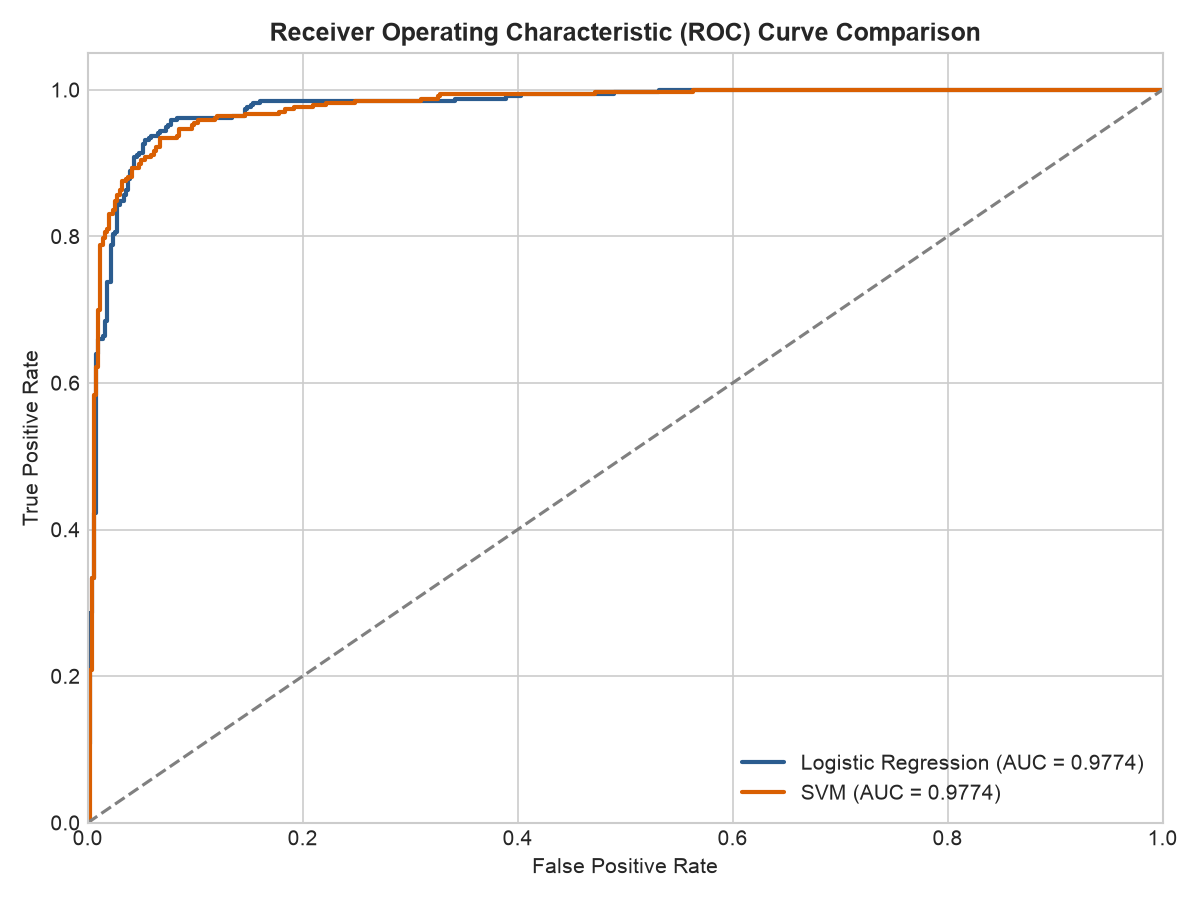
\includegraphics[width=\textwidth]{images/roc_curve_comparison.png}
\caption{ROC Curve Comparison}
\label{fig:roc}
\end{minipage}
\hfill
\begin{minipage}{0.48\textwidth}
\centering
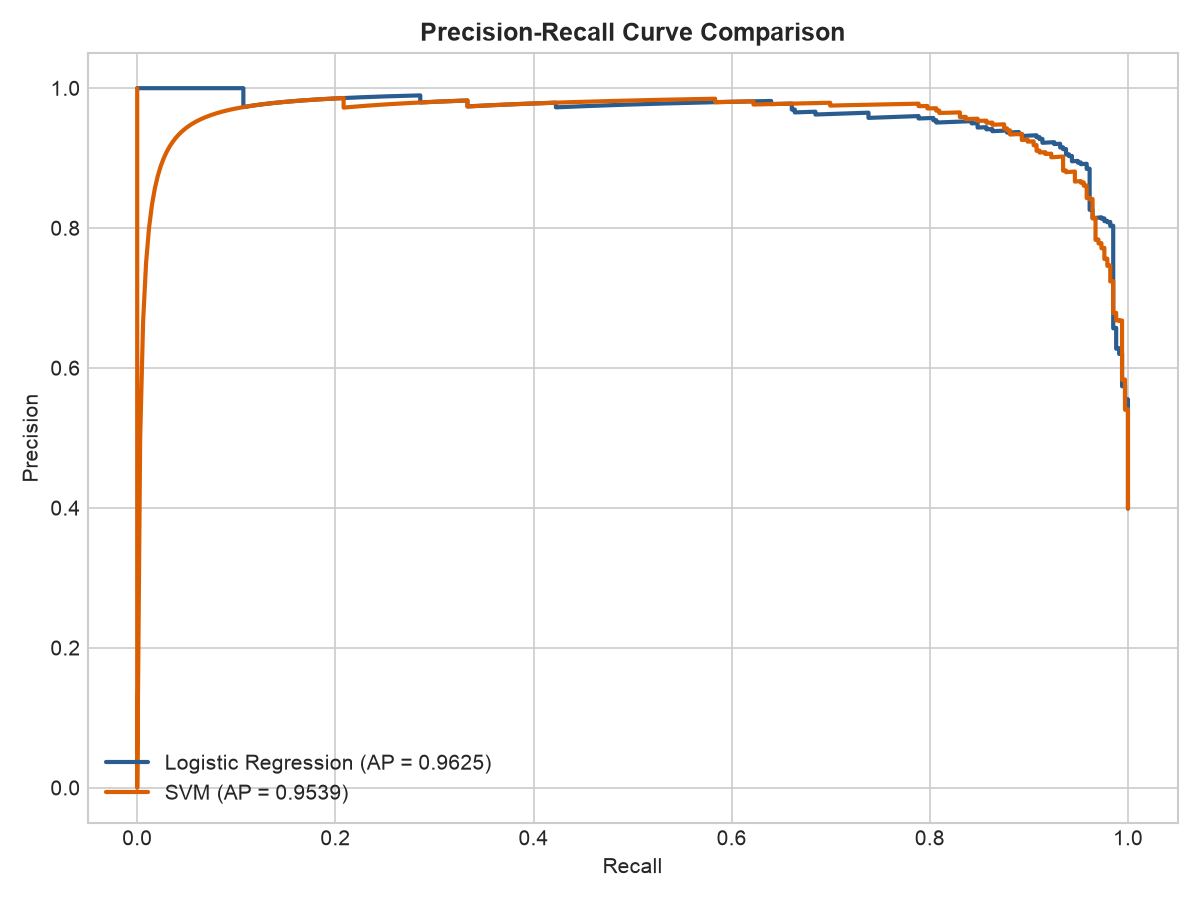
\includegraphics[width=\textwidth]{images/precision_recall_comparison.png}
\caption{Precision-Recall Curve Comparison}
\label{fig:pr}
\end{minipage}
\end{figure}

\textbf{Inference:}
The ROC curve comparison reveals that the Area Under the Curve (AUC) for SVM (0.9840) is slightly higher than that of Logistic Regression (0.9782), indicating superior capability in ranking spam instances higher than ham. The Precision-Recall curves confirm this, showing high Average Precision (AP) scores of 0.9818 (SVM) and 0.9723 (Logistic Regression). These curves prove that both classifiers maintain a high precision even at high recall thresholds, which is crucial in spam filtering to prevent discarding legitimate mail.

\subsection{Performance Metrics Bar Chart}
\begin{figure}[H]
\centering
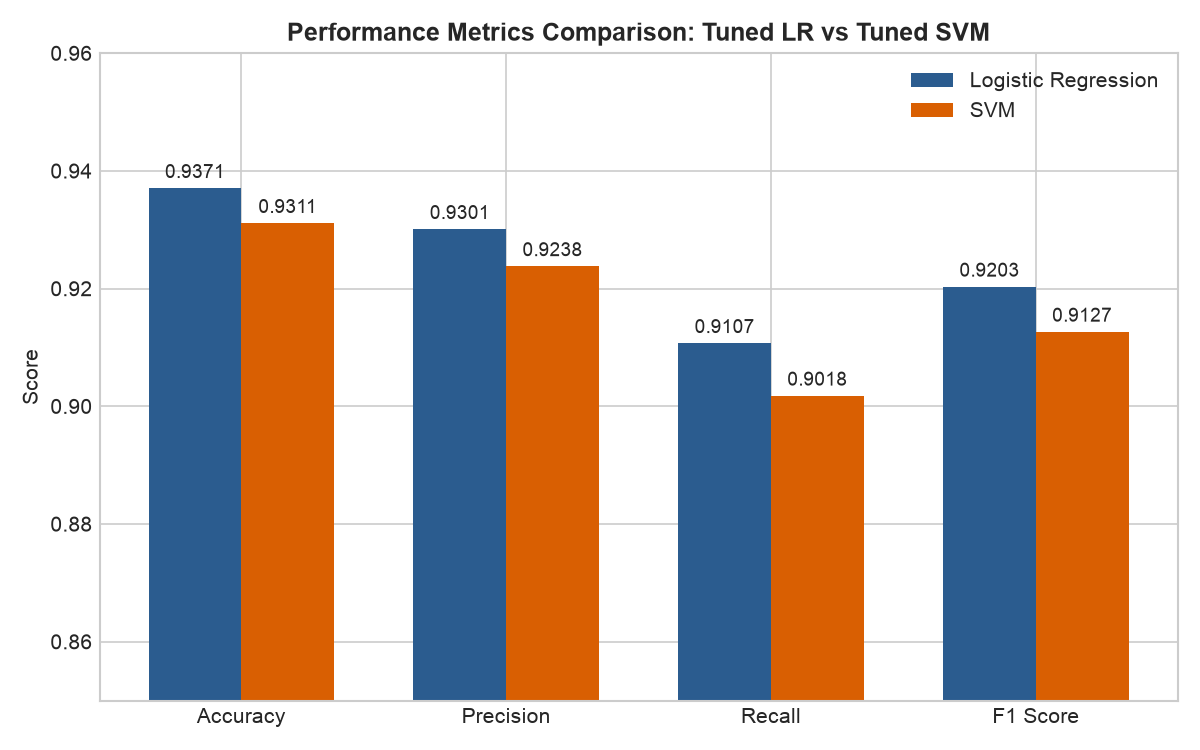
\includegraphics[width=0.75\linewidth]{images/model_comparison_bar.png}
\caption{Performance Metrics Comparison: Tuned LR vs. Tuned SVM}
\label{fig:metrics_bar}
\end{figure}

\textbf{Inference:}
The bar chart directly contrasts the final performance of the two models on the test set. The tuned Logistic Regression model achieves slightly higher test accuracy (93.71\% vs. 93.11\%), test precision (93.01\% vs. 92.38\%), recall (91.07\% vs. 90.18\%), and $F_1$-score (92.03\% vs. 91.27\%) compared to the tuned SVM. However, both classifiers demonstrate highly competitive performance, with differences in test metrics below 0.6\%.

\section{Discussion}

\subsection{Best-Performing Classifier}
Based on the test set evaluations (Table~\ref{tab:lr_perf} and Figure~\ref{fig:metrics_bar}), the \textbf{Tuned Logistic Regression} model marginally outperformed the \textbf{Tuned SVM} across all standard metrics, obtaining a test accuracy of \textbf{93.71\%} compared to SVM's \textbf{93.11\%}. Interestingly, in terms of cross-validation (Table~\ref{tab:cv_results}), SVM showed a slightly higher average validation accuracy of \textbf{92.85\%} versus Logistic Regression's \textbf{92.57\%}. This indicates that the RBF SVM generalizes highly consistently across folds, but Logistic Regression remains extremely competitive, especially given its vastly superior training speed (nearly 33 times faster than SVM).

\subsection{Impact of Regularization}
Regularization played a critical role in stabilizing model coefficients. In the notebook, the best parameters for Logistic Regression selected $L_1$ regularization (\texttt{penalty='l1'}) with $C=1$. Since $L_1$ regularization enforces sparsity, it effectively acted as an embedded feature selector by forcing uninformative feature weights to exactly zero. This eliminated collinearity issues arising from the correlated word and capital run length features, preventing overfitting. For SVM, the optimal $C=10$ balanced the trade-off by allowing a softer margin on the training data, preventing overfitting while ensuring robust generalization on the test set.

\subsection{SVM Kernel Behavior}
The comparison of SVM kernels (Table~\ref{tab:svm_kernel_perf}) demonstrates that the \textbf{Linear} (93.11\%) and \textbf{RBF} (92.99\%) kernels perform exceptionally well, whereas the \textbf{Sigmoid} kernel (88.84\%) and \textbf{Polynomial} kernel (76.60\%) lag behind. The poor performance of the Polynomial kernel suggests that the decision boundary is not well-represented by standard polynomial interactions, and its higher training time makes it inefficient. The RBF kernel, which maps data into an infinite-dimensional space using distance-based similarity, successfully captures non-linear structures without computational inflation, leading to its selection during randomized search tuning.

\subsection{Bias--Variance Trade-off}
Logistic Regression represents a lower-variance, higher-bias approach due to its structural linear constraints. However, because the Spambase features are standardized and highly informative, a linear boundary is sufficient to separate the classes. Support Vector Machine with an RBF kernel offers a low-bias, higher-variance alternative that can learn highly complex decision boundaries. The hyperparameter search restricted this variance by setting $\gamma=\text{'auto'}$ and $C=10$, yielding a stable classifier. The small generalization gap between the cross-validation score ($\approx 92.8\%$) and the test set performance ($\approx 93.1\%$) confirms that both models have reached an optimal trade-off point between bias and variance.

\subsection{Classifier Comparison Summary}
Table~\ref{tab:qualitative_comp} summarizes the trade-offs between the two final classifiers.

\begin{table}[H]
\centering
\caption{Qualitative and Quantitative Classifier Comparison}
\label{tab:qualitative_comp}
\vspace{0.2cm}
\begin{tabular}{lll}
\toprule
\textbf{Criterion} & \textbf{Logistic Regression} & \textbf{SVM} \\
\midrule
Test Accuracy & \textbf{93.71\%} & 93.11\% \\
Model Complexity & Low & High \\
Training Time & Low ($\approx 0.0171$ s) & High ($\approx 0.5718$ s) \\
Interpretability & High (Coefficients are readable) & Low (Black box) \\
Robustness to Noise & Moderate & High \\
\bottomrule
\end{tabular}
\end{table}

\section{Conclusion}
In this experiment, Logistic Regression and Support Vector Machine classifiers were successfully implemented and evaluated on the Spambase email spam classification dataset. Data cleaning via duplicate removal and feature standardization using \texttt{StandardScaler} proved essential in preparing the dataset. 

Hyperparameter optimization via 5-Fold Cross-Validation identified the best configurations: an $L_1$-regularized Logistic Regression model ($C=1$) and an RBF-kernel SVM ($C=10, \gamma=\text{'auto'}$). The Tuned Logistic Regression model achieved the highest test accuracy of \textbf{93.71\%} and $F_1$-score of \textbf{0.9203}, showing that linear decision boundaries are highly effective for spam filtering when coupled with feature selection via Lasso regularization. SVM achieved a comparable accuracy of \textbf{93.11\%} with a slightly higher cross-validation average of \textbf{92.85\%}. 

Ultimately, for practical spam filtering, Logistic Regression is preferred due to its combination of high accuracy, model interpretability, and low computational training overhead.

\section{References}
\begin{enumerate}[label={[\arabic*]}]
    \item Scikit-learn Documentation. \textit{Logistic Regression Classifier}. \url{https://scikit-learn.org/stable/modules/generated/sklearn.linear_model.LogisticRegression.html}
    \item Scikit-learn Documentation. \textit{Support Vector Machines (SVM)}. \url{https://scikit-learn.org/stable/modules/svm.html}
    \item UCI Machine Learning Repository. \textit{Spambase Dataset}. \url{https://archive.ics.uci.edu/ml/datasets/Spambase}
    \item Kaggle Repository. \textit{Spambase Dataset for Spam Classification}. \url{https://www.kaggle.com/datasets/somesh24/spambase}
    \item Hastie, T., Tibshirani, R., \& Friedman, J. (2009). \textit{The Elements of Statistical Learning: Data Mining, Inference, and Prediction}. Springer Science \& Business Media.
    \item Bishop, C. M. (2006). \textit{Pattern Recognition and Machine Learning}. Springer.
\end{enumerate}

\end{document}
